



\vspace{-2mm}



%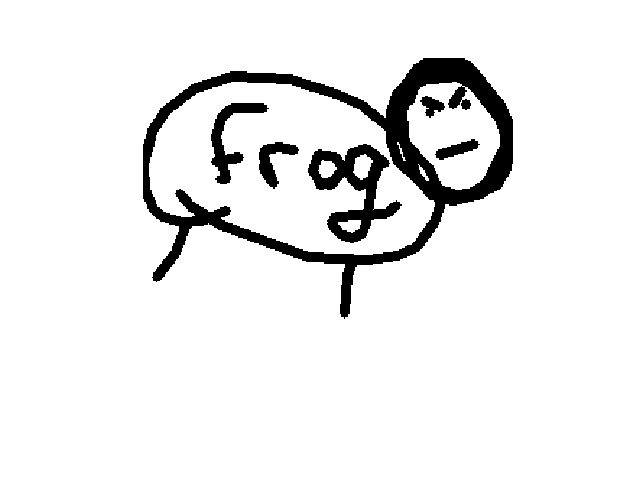
\includegraphics[width=0.5\textwidth]{figures/frog_draw_2.png}
%test texte

\begin{center}
Transformation de vecteurs de traits de crayon (position x, y)  en photos.
\end{center}

\begin{center}

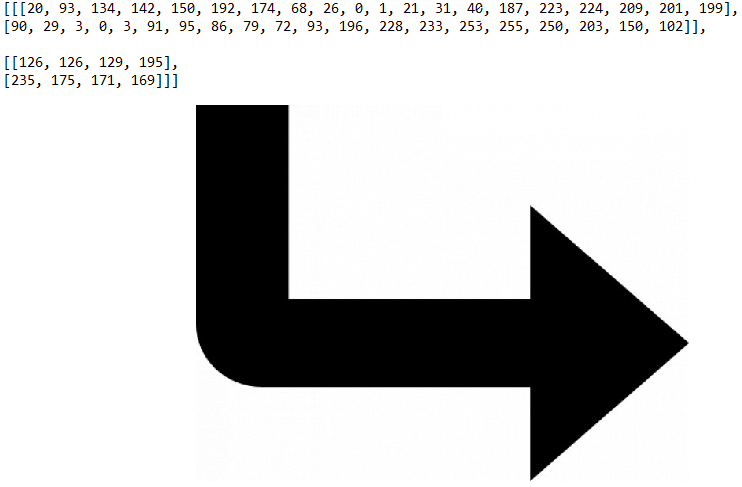
\includegraphics[width=15cm,height=15cm,keepaspectratio]{figures/vecteur_fleche.png}
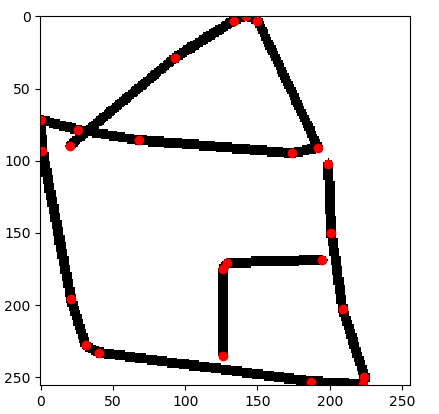
\includegraphics[width=15cm,height=15cm,keepaspectratio]{figures/housedraw.png}
%\captionof{figure}{Transformation des vecteurs }
\end{center}




\vspace{4mm}




\centering
\begin{itemize}
\item Images très différentes pour une même classe
\item Certaines images incomplètes
\end{itemize}

\vspace{4mm}
\begin{center}
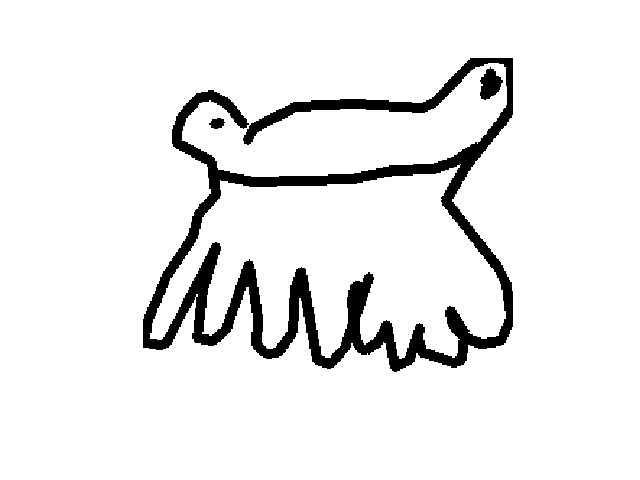
\includegraphics[width=9cm,height=9cm,keepaspectratio]{figures/frog_draw_1.png}
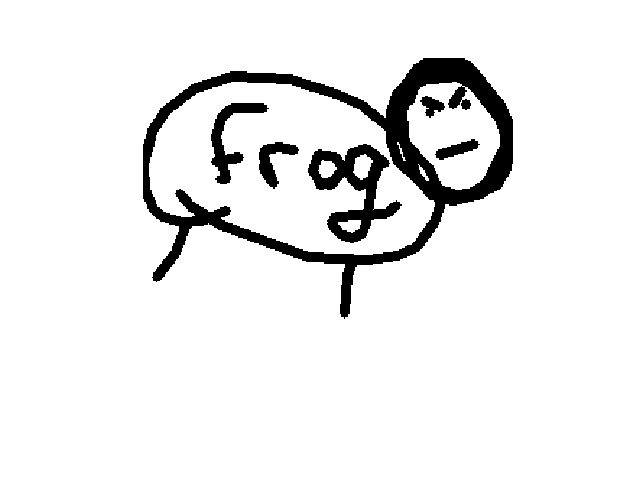
\includegraphics[width=9cm,height=9cm,keepaspectratio]{figures/frog_draw_2.png}
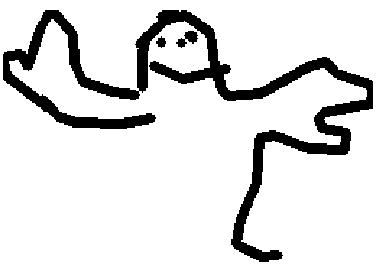
\includegraphics[width=9cm,height=9cm,keepaspectratio]{figures/frog_draw_3.png}

\includegraphics[width=9cm,height=9cm,keepaspectratio]{figures/frog_draw_4.png}


\end{center}




























